\section{Elliptic Curves key pair generation}
The public/private key pair generation is done by using elliptic curves for performance and memory complexity reasons (at a fixed security level the EC keys are more than 10 times shorter compared to the RSA/DSA/ElGamal ones): a message in Android has a maximum length of 140 characters (bytes), so we had no choice if we didn't (and we didn't since it would have screwed up our crypto layer) want to use multipart messages. The curve used is a NIST standard: "secp256r1", also known as "prime256v1", which generates 256 bits long keys (we actually thought to use "secp521r1" for enhanced security, but the keys were too long). Using a named curve which is also a standard has a few advantages: first, it generates automatically all the parameters needed, second, its security has been widely tested by the cryptanalists of all the world. The generated keys are encoded into byte arrays in different ways: the private ones using the "PKCS8 encoded key specifiers", the public ones with the "X509 encoded key specifiers". It's always possible with a key factory to decode both encodings leading to keys identical to the pre-encoding ones. The keys are generated this way: given the order of the EC group and a randomly chosen point of the curve (different from the one at infinity), which is also a generator of the group, the private key is that point and the public key is computed as [priv]P, where the multiplication denoted by [integer]Point is reduced to a sequence of application of doubling a point and addition between two points. The pictures below shows graphically how these operations are defined for elliptic curves.\\

\vspace{1cm}
\begin{center}
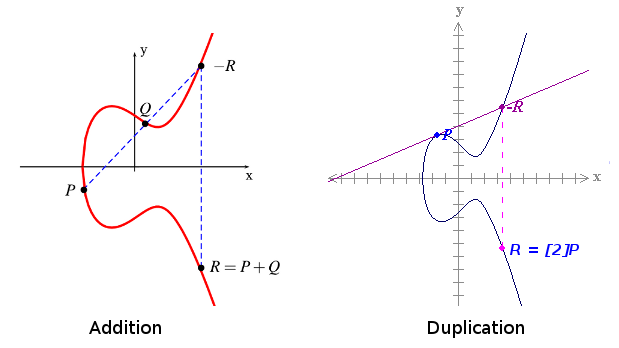
\includegraphics[scale=0.5]{images/ec}\\

\vspace{1cm}
EC points addition and doubling\\
\end{center}